\chapter{NoSQL e OrientDB}

\section{Il movimento NoSQL}
Prima di parlare di OrientDB è necessario introdurre il concetto di \emph{database non relazionale} e spiegare il come ed il perchè del movimento NoSQL.

\subsection{Un pò di storia}
Possiamo rilevare che la prima comparsa del termine NoSQL, sia riconducibile ad un italiano, Carlo Strozzi, che, sul finire degli anni '90, ideò un database, lo \emph{Strozzi NoSQL}, che non si avvaleva della sinstassi SQL per accedere ai dati memorizzati. Nonostante ciò non è possibile rilevare in questo lavoro alcuna caratteristica che sia precorritrice dell'attuale \emph{movimento} NoSQL.

La nascita formale del movimento è datata 11 giugno 2009. All'epoca già esistevano dei database che non si basavano sul modello relazionale dei dati, principalmente stiamo parlando di BigTable (da Google), e di Dynamo (da Amazon), e che avevano ispirato il lavoro di altri informatici (portando alla nascita di colossi quali MongoDB, Cassandra e Voldemort), ma non avevano ancora una loro collocazione precisa. 
In tale data Johan Oskarsson si trovava a San Francisco per un metting su 
Hadoop\footnote{Framework, rilasciato con licensa open source e sviluppato in Java, che permette il calcolo distribuito scalando da un server fino a migliaia di macchine. Il pacchetto include, oltre ai pacchetti base: un file system distribuito (HDFS), un framework per il job scheduling e la gestione delle risorse ed un sistema per l'elaborazione parallela.} 
ed in tale occasione decise di organizzare lui stesso un convegno sulle novità che il mondo dei database stava vivendo.

Il nome di questo talk doveva essere breve, significativo e con pochi risultati su Google, così che una successiva ricerca permettesse di trovare senza difficoltà i riferimenti a questo storico metting. Così, dopo una breve consultazione online, si optò per NoSQL, nome proposto da Eric Evans sul canale IRC di Cassandra. La ricerca degli interventi che si sarebbero succeduti durante il meeting richiedeva che i database presentati fossero \emph{open-source}, \emph{distribuiti} e \emph{non relazionali}. Durante questo \emph{Woodstock} si discusse delle nuove tecnologie emergenti: Voldemort, Cassandra, Dynomite, HBase, Hypertable, CouchDB e MongoDB.  

\subsection{Perchè NoSQL}
Il termine NoSQL sebbene sia un termine forte, che colpisce, come venne riconosciuto già all'epoca del meeting, non determina in positivo i database che a questa categoria appartengono. Piuttosto descrive tutto ciò che un database NoSQL \emph{non} è.

A tutt'oggi non esiste una definizione standardizzata di NoSQL; non si è neppure concordi su quale sia il significato da attribuire a questo acronimo: c'è chi sostiene che NoSQL sia l'acronimo di Non SQL, e c'è chi sostiene, e sono sempre di più, che sia l'acronimo di Not only SQL.
Secondo l'autore di questo testo, l'interpretazione corretta da attribuire a NoSQL è la prima, ossia Non SQL: a tal proposito si noti che, se così non fosse, la sigla sarebbe stata NOSQL.

Tuttavia è possibile individuare nel mondo del NoSQL delle caratteristiche condivise, seppur con delle eccezioni, da tutti i facenti parte di questa categoria:
\begin{itemize}
\item \emph{Rinuncia all'SQL}. Evidentemente i database NoSQL non fanno uso di SQL, sebbene alcuni di essi offrano all'utente un'interfaccia SQL-like per rendere più dolce il passaggio dai database relazionali a quelli non relazionali (Cassandra, con CQL, ne è un esempio).
\item \emph{Progetti open-source}. Come richiesto da Johan, i database NoSQL dovrebbero essere open-source. Attualmente la maggior parte di essi sono open-source, ed offrono assistenza a pagamento, o versioni definite \emph{Enterprise}, ovvero versioni con dei tool di gestione avanzati non disponibili se non pagando una licenza.
\item \emph{Scalabilità}. Quasi la totalità dei database NoSQL offre la capacità di scalare orizzontalmente, piuttosto che verticalmente. Torneremo su questo argomento nei paragrafi successivi.
\item \emph{Tempistiche}. Questo è l'unico punto che viene condiviso da tutti: solo i database nati nel XXI secolo sono definiti NoSQL, in quanto nati con lo scopo di soddisfare le necessità che in questo periodo si sono manifestate. Tutti i database non relazionali nati nel XX secolo vengono chiamati \emph{BC}, acronimo di 
\emph{Before Codd}\footnote{Edgar Frank "Ted" Codd, informatico inglese che, durante la sua esperienza lavorativa presso la IBM, ideò il modello relazionale per la gestione delle basi dati relazionali.}
\item \emph{Schema-less}. La quasi totalità dei database non relazionali permette di lavorare in modalità \emph{schema-less}, ovvero senza uno schema fisso da rispettare. Questo permette di aggiungere campi ai record senza necessità di modificare lo schema. Questa caratteristica è particolarmente utile nelle situazioni in cui si ha una non uniformità dei dati, situazione che in database relazionale costringe ad un inutile spreco di spazio. Non si deve pensare, però, che non sia possibile definire, \emph{volutamente}, uno schema da rispettare: ci sono database non relazionali che permettono di operare in modalità \emph{schema-full} - orientDB è uno di questi.
\end{itemize}

Torniamo ora sul termine NoSQL: i sostenitori del "Not only SQL", seppur errando nell'interpretazione dell'acronimo, hanno perfettamente capito qual'è lo spirito di questo movimento: non si ha una tecnologia specifica, un pattern con cui risolvere dei problemi. Piuttosto abbiamo una classe di soluzioni, un \emph{set} di possibilità, l'una diversa dalle altre. A tal proposito, va sottolineato che NoSQL non significa rinnegare l'SQL, ne abbandonarlo. Tutt'altro: il 90\% dei problemi di persistenza potrebbe essere risolto usando dei database relazionali.

Va capito che partecipare al movimento NoSQL significa ampliare le proprie possibilità, avere delle soluzioni innovative e \emph{specifiche} per il problema in questione: \emph{i database relazionali sono una possibilità per il data storage, e non la soluzione}. Questo approccio alla persistenza viene detto \emph{polyglot persistence}.

Bisogna sottolineare che, proprio per il periodo che li ha visti nascere, i database NoSQL rappresentano, come abbiamo visto sopra, la soluzione ideale per lo storage di grandi dimensioni di dati o per la divisione su più macchine (sia con lo \emph{sharding}, che con la replicazione, sia essa \emph{multi-master} o \emph{master-slave}), rendendoli la soluzione ideale per applicazioni web.

Come abbiamo visto, i database NoSQL offrono caratteristiche non omogenee, ed in base a come operano è possibile riconoscere delle classi:
\begin{itemize}
\item \emph{Document store}. Il concetto centrale è il documento, che incapsula i dati e li codifica in uno standard che può essere, tra gli altri, l'XML, il JSON o il BSON.
\item \emph{Grafi}. Questo tipo di database è ottimale per soluzioni in cui tra i dati intercorrono un numero non predeterminato di relazioni, come nel caso dei social network, o delle mappe stradali.
\item \emph{Key-Value store}. Il database memorizza i dati senza schema, e e permette il loro recupero attraverso una chiave, come nelle hashmap.
\item \emph{Object database}. Il database memorizza dei veri e propri oggetti.
\item \emph{RDF database}. Il database memorizza le informazioni e le cataloga in base ai loro metadati, così come specificato dal RDF\footnote{Resource Description Framework, standard definito dal W3C}.
\end{itemize}

\subsection{NoSQL ed il teorema CAP}
Quando si ha a che fare con un database, a causa di un teorema, detto \emph{teorema CAP}, bisogna sempre sapere, prima di fare una scelta, sapere cosa si vuole ottenere.

Prima di tutto, però, analiziamo questo teorema, diventato tale nel 2002, quando S. Gilbert e N. Lynch dimostrarono la congettura di E. Brewer, risalente al 2000. Esso afferma che in un sistema distribuito è impossibile soddisfare contemporaneamente tutte e tre le seguenti garanzie:
\begin{itemize}
\item \emph{Consistenza} (tutti i nodi vedono gli stessi dati nello stesso momento).
\item \emph{Disponibilità} (ogni richiesta deve ricevere una risposta su ciò che è andato a buon fine e su ciò che non lo è)
\item \emph{Tolleranza alla partizione} (il sistema continua a funzionare nonostante un arbitrario numero di messaggi venga perso o ci sia un problema in una parte del sistema)
\end{itemize}

In base a quale garanzia si decide di abbandonare, si avrà un sistema definito ACID o un sistema definito BASE. Nel primo caso, ACID è l'acronimo di Atomico, Consistente, Isolato, Duraturo, e, come sembra evidente, questo tipo di database garantisce una sicurezza senza pari, compromettendo, però, le prestazioni e la disponibilità.

Al contrario, un sistema BASE, coerentemente con suo significato (consistenza effettiva, soft-state, fondamentelmente disponibile), risulta essere orientato alle performance ed alla disponibilità parallela, a scapito della coerenza.

Attualmente i database relazionali incarnano il principio ACID, e risulta possibile una scalabilità verticale, ovvero aggiungere risorse (ad esempio CPU) ad un singolo server, su cui è mantenuto il database, mentre i database non relazionali, per la maggior parte, incarnano il principio BASE, rendendo possibile la scalabilità orizzontale, ovvero aggiungere risorse in parallelo, quindi distribuire il database su più macchine ed incrementare le prestazioni parallelizzando l'elaborazione. OrientDB, ad esempio, permette di scegliere quale approccio utilizzare, introducendo il concetto di \emph{transazione atomica}.

\section{Introduzione ad OrientDB}
OrientDB nasce nel 2010 per opera di Luca Garulli, già autore, presso Asset Data, di Roma Framework. Come database NoSQL si caratterizza per le sue prestazioni e per la portabilità, derivante dal fatto di essere completamente scritto in Java e di non dipendere da librerie esterne, oltre che per le sue dimensioni estremamente ridotte: il pacchetto, completo di API, si aggira intorno ai 6MB.
Il suo punto di forza è la versatilità, potendo gestire diverse modalità:
\begin{itemize}
\item \emph{Grafo} o \emph{Documentale}. L'utente decide che tipologia di database creare al momento dell'inizializzazione, se documentale o a grafo.
\item \emph{Transazionale} o \emph{non transazionale}. L'utente decide al momento della stesura del codice che si interfaccia con il database se usare le transazioni, rendendo l'ambiente performante nel caso di un ambiente client-server che richiede continue modifiche sui dati, o di non usarle, effettuando i salvataggi ad ogni modifica.
\item \emph{Schema-less} o \emph{schema-full} o \emph{mixed}. L'utente decide se impostare uno schema predefinito, se lavorare senza vincoli, o se impostare per alcuni elementi un vincoli, e lasciare liberi altri. Tutto ciò anche a database popolato.
\item \emph{Local} o \emph{embedded} o \emph{in memory}. L'utente, all'atto della creazione dell'istanza, decide se creare un database remoto, con cui sarà possibile comunicare solo tramite server, locale, con cui sarà possibile comunicare usando direttamente le API fornite, senza necessità di un server attivo (come SQLite) o in modalità in memory, salvando, cioè, i dati in RAM, ed accedendovi solo tramite API.
\end{itemize}

Oltre a ciò non va tralasciata la potenza di OrientDB, che si basa su un innovativo algoritmo di indicizzazione, definito MVRB-tree (multi value red black tree), derivato dai red-black tree e dai B+tree con i benefici di entrambi, che permette di raggiungere i 150000 record memorizzati al secondo\footnote{testato su un HP Pavillon dv6 con Intel Core i7 720q, 4GB RAM e HDD E-SATA 7200rpm}, e la sua predisposizione ad un ambiente web, con il supporto nativo ad HTTP e Rest.

Infine, da segnalare la presenza di una sintassi SQL-like che permette la migrazione facilitata da un RDBMS ad OrientDB.

\section{L'architettura di OrientDB}
\subsection{Lo storage fisico}
Come abbiamo precedentemente visto, OrientDB può funzionare con tre tipi di storage: in maniera locale, ed in questo caso l'accesso al database avviene dallo stesso processo che lo ha richiesto, rendendo impossibile l'aprtura dello stesso da parte di un altro processo; in maniera remota, ed in questo caso l'accesso avviene attraverso il server, che risiede su un processo distinto da quello del richiedente, mediante il protocollo REST, permettendo di gestire anche l'accesso concorrente; in memory, ovvero tutti i dati rimangono in RAM, e nessun dato viene scritto su file system.

Come avviene realmente lo storage dei dati su disco? OrientDB ha tre strutture di storage separate, che si riflettono poi sull'indirizzazione dei record, come vedremo successivamente. La prima, presente per garantire che si usino le transazioni sicure, è detta \emph{TxSegment}, ed è quella parte che si occupa di fare il logging dei cambiamenti avvenuti e che, in caso di fallimento, si occupa di fare il \emph{rollback} dei dati.

La seconda separa i dati in \emph{Cluster}, ovvero un gruppo molto generico di dati raggruppati o in base al loro tipo (ad esempio il cluster 'Seas' potrebbe contenere tutti i record dei vari mari) o in base a dei valori (ad esempio il cluster 'hotelDiLusso' potrebbe contenere tutti gli hotel che hanno 4 o più stelle). OrientDB usa due o più file per gestire i cluster: uno o più file con estensione .ocl che contengono i puntatori ai record effettivi, ed uno ed un solo file con estensione.och che contiene gli \emph{hole}, ovvero puntatori a record eliminati e che possono essere dunque rimpiazzati o deframmentati.

Infine abbiamo i \emph{Data segment}, ossia i file che poi, concretamente, rappresentano il contenuto di ciascun record. Come per i cluster, i data segment necessitano di due o più file, almeno uno con estensione .oda, che contiene i record, ed uno ed un solo file con estensione .odh che contiene gli hole.

\begin{figure}
\centering
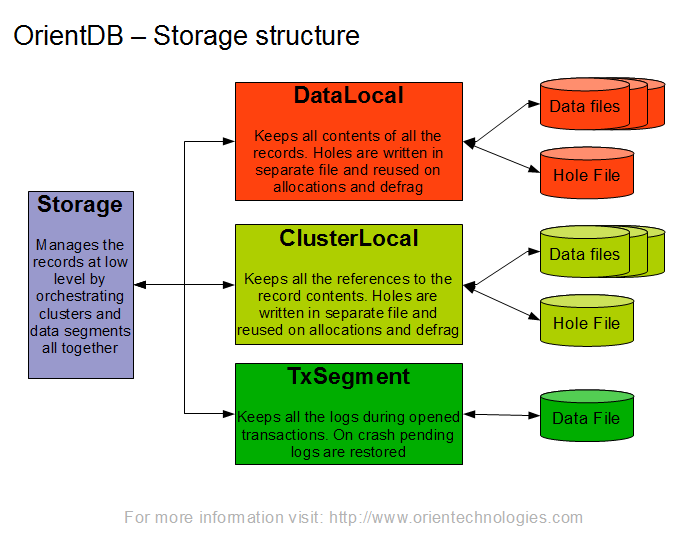
\includegraphics[scale=0.5]{./orient.png}
\caption{Schematizzazione dell'architettura del data storage di OrientDB}
\label{fig:1}
\end{figure}

Ciascun record in OrientDB ha un identificatore univoco, chiamato \emph{RecordID}, noto anche con l'acronimo RID. Esso è nella forma \#<cluster>:<position>, dove cluster è l'ID del cluster considerato e position è la posizione assoluta del record nel cluster. Entrambi i numeri sono positivi, tranne nel caso si stiano trattando record temporanei (come nelle transazioni): il tal caso avremo numeri negativi. I RID in OrientDB sono univoci, e quindi non sarà necessario fornire i documenti di chiavi primarie come in un database relazionale.

Ciò detto, come si può vedere in figura 2.2, quando ad OrientDB viene richiesto un record si attiva il seguente processo: l'utente chiede il record \#x:y, il database verifica che effettivamente l'utente abbia i permessi sufficienti per caricare il record richiesto, se si, lo storage chiede al Cluster x dove si trovi il file y, e questo gli risponderà specificando \emph{offset}, \emph{dimensione}, \emph{tipo} e \emph{versione}; a questo punto lo storage interrogherà il file corretto, leggendo i byte interessati e restituendoli al database che, a sua volta, li restituirà all'utente.
\begin{figure}
\centering
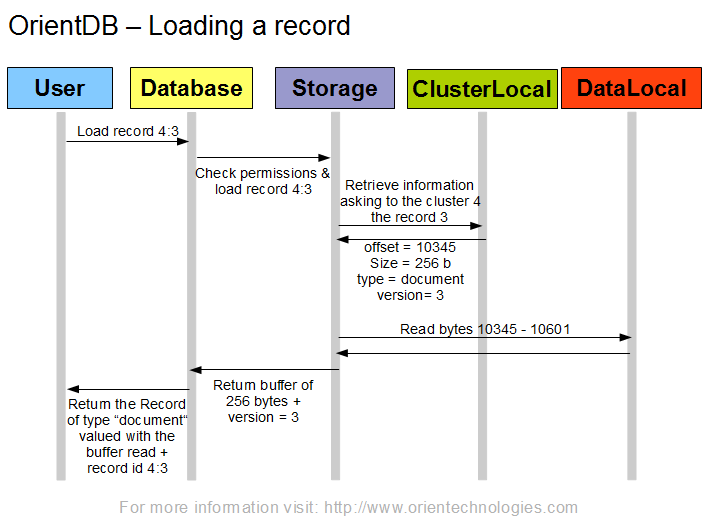
\includegraphics[scale=0.5]{./orientFlow.png}
\caption{Flusso generato da OrientDB per rispondere alla richiesta di un record}
\label{fig:2}
\end{figure}

\subsection{Lo storage logico}
L'unità fondamentale dello storage logico di OrientDB è la classe, intesa come ci si aspetterebbe, ovvero come concetto preso dall'Object
Oriented paradigm. A livello fisico, una classe corrisponde ad un tipo di record: quindi creare una classe equivale a creare un cluster.
In OrientDB è prevista l'eredità delle classi, ovvero è possibile creare una sottoclasse che estende una classe già esistente e ne eridita tutti gli attributi. Poichè potrebbe rendersi necessario creare classi che non hanno effettivamente dei record, ma che fungono da superclasse, è stato previsto dagli sviluppatori un meccanismo per definire astratta una classe, ed evitare di creare cluster inutili.

Come abbiamo anticipato, OrientDB fornisce il supporto alla sintassi SQL, ed in questo caso le classi devono essere utilizzate come fossero tabelle, o, in alternativa, al posto del nome di classe è possibile usare l'id del cluster cui la classe fa riferimento.

La cosa interessante dei database non relazionali che lo scrittore ha dato per scontato nella trattazione introduttiva al mondo NoSQL, è il fatto che non si ha più il vincolo dell'atomicità dei valori. Questo permette ad OrientDB di ottimizzare le relazioni tra record, introducendo il concetto di \emph{relazione}:
\begin{itemize}
\item \emph{Referenziata}. In questo caso vengono salvati nel documento link diretti agli elementi con cui il documento stesso è in relazione, permettendo il caricamento senza costose JOIN tra tabelle. Questo tipo di relazione è bidirezionale in quanto ciascun record conserva il RID del record con cui è in relazione.
\item \emph{Embedded}. In questo caso i record embedded sono contenuti nel record che li incorpora. E' una relazione forte, rappresentabile come una relazione di composizione UML. In questo caso il record embedded non ha un RID, dal momento che non può essere referenziabile da nessun altro record, ed è accessibile solo dal record contenitore. Se si elimina il record esterno automaticamente vengono eliminati ricorsivamente anche tutti i record embedded.
\end{itemize}

\endinput

